\chapter[Synthesis]{Synthesis}
\label{cha:Chapter6}
\newpage

This thesis aims to contribute towards efforts made in large-scale land cover mapping, with an emphasis on the benefits of combining several datasets from different sources and of different types. It presents different steps of a methodology to extract training data from multiple rich human-annotated datasets and overlay them on Earth observation data from diverse sources. It furthermore details the challenges and benefits of creating land cover maps that navigate the trade-off between spatial, temporal, and thematic resolution, as well as quantity and allocation accuracy.

This thesis, especially in its first two chapters, describes a relatively applied line of research. Besides the chapters themselves, several datasets were produced, and have been published as open data (CC-BY):
\begin{enumerate}
    \item 2000-2020 quarterly Landsat composites at 30m resolution and 7 bands (on \url{stac.ecodatacube.eu});
    \item 2016-2019 quarterly/annual Sentinel-2 composites at 10-30m resolution, depending on the band (on \url{stac.ecodatacube.eu});
    \item Input dataset for gap filling and land cover mapping using the eumap library \citep{parente2020input};
    \item An Ensemble Digital Terrain Model of Europe at 30m resolution \citep{hengl2021continental}
    \item 2000-2019 annual Land Use / Land Cover maps of Europe at 30m resolution and 43 classes \citep{parente2021continental};
    \item Five annual land cover maps of five European countries (Belgium, Czechia, Germany, Luxembourg and The Netherlands) at 30m resolution and 8 classes, whose class proportions match Eurostat area estimates \citep{witjes2024iterative_data}.
\end{enumerate}
The third chapter of the thesis describes relatively more innovative attempts to model land cover in a way that is faithful to area estimates. The proposed algorithm (IMP) may have further uses and implications, these will also be discussed in this synthesis chapter. It is divided into two sections: the first summarizes contributions to the research objectives formulated in Section~\ref{sec:research_objectives} and the second section reflects on these contributions, offering perspectives on future research opportunities. 

\section{Main Findings}
    The chapters of this thesis each address multiple research questions and should be considered jointly in this synthesis. Their results will be discussed from the perspective of the research questions; each question is discussed below.
    
    \subsection{What are the benefits and challenges of combining multiple large time-series and static EO datasets into Analysis-Ready Data for the purpose of land cover classification?}
    \label{syn:rq1}

        This research question was largely explored in Chapters\@~\ref{cha:chapter2}\@~and\@~\ref{cha:chapter3}. Chapter\@~\ref{cha:chapter2} details the construction of an Earth observation data cube from various sources (Landsat, Sentinel-2 and several DTMs), and includes experiments that investigate the performance of land cover models using different combinations of these datasets. Chapter\@~\ref{cha:chapter3} uses most of this data cube to train a single LULC classification model, which is subsequently used to create annual maps of Europe between 2000 and 2019. 

        \subsubsection{Benefits}
    
            Our land cover experiments in Chapter\@~\ref{cha:chapter2} show that random forest models trained on the largest combination of datasets achieved the highest classification accuracy during cross-validation and that models trained on Landsat and DTM data achieved the highest accuracy on test data. This is in line with other work reporting that including auxiliary variables in the feature space can improve performance \citep{zhu2016optimizing, hurskainen2019auxiliary, hosseiny2022urban, santos2012multiscale}.

            Chapter\@~\ref{cha:chapter2} also details the creation of an Ensemble DTM which was more accurate than its four source datasets, with a RMSE 6.544 vs RMSE of 8.451-9.900. This demonstrates that in the case of continuous variables, different versions or representations of that variable can be used as input for a machine learning algorithm, and that the predictions by this algorithm can be more accurate.
            
            In Chapter\@~\ref{cha:chapter3}, the top 15 most important variables of the ensemble land cover model contain data from six sources: several bands from two satellite programs (Landsat and MODIS), long-term probability of surface water occurrence \citep{pekel2016high}, geometric temperature \citep{kilibarda2014spatio}, multiple DTM variables, and the cost distance to the nearest coastline (see Figure~\ref{fig:variable_importance}). 
    
        \subsubsection{Challenges}
            
            Experiments in Chapter\@~\ref{cha:chapter2} showed that models using the full feature space (Landsat, Sentinel-2 and DTM) achieved the highest classification accuracy, with different datasets improving the results for different land cover classes. This is supported by variable importance in Chapter \ref{cha:chapter3}: data from four different sources (Landsat, surface water frequency, DTM, and distance to coast) were among the top 15 of 200 variables for LULC modeling.
            
            While it is clear that combining different datasets into one feature space can improve model performance, there are some challenges:
    
            \textbf{Spatial resolution}: Overlaying different raster datasets onto training samples may yield high accuracy (like in Chapter\@~\ref{cha:chapter2}), but can cause artifacts in the shape of low-resolution raster cells when creating maps at the highest resolution among the used datasets. Fortunately, recent findings suggest that certain modeling techniques, such as convolutional neural networks, can counteract this effect \citep{robinson2019large}. In Chapters\@~\ref{cha:chapter3}\@~and\@~\ref{cha:chapter4}, we used low-resolution MODIS data as part of the feature space. To avoid artifacts, we smoothed it while resampling it to a 30~m resolution, but this is a very unsophisticated method and may have led to the loss of a lot of explanatory power. This is also reflected by its low position in the variable importance of the ensemble model in Chapter\@~\ref{cha:chapter3}.

            \textbf{Temporal resolution} can be subdivided into the temporal resolution of the feature space and that of the mapped units. It is essential to have a high temporal resolution in the feature space to correctly detect and distinguish different vegetation types due to the temporal dynamics of their phenology. 
            
            The time range represented by a single map has different implications for the accuracy of different classes. In Chapters\@~\ref{cha:chapter3}\@~and\@~\ref{cha:chapter4}, we chose to make annual maps, and in Chapter\@~\ref{cha:chapter3}, we made annual maps for each consecutive year. This does not work equally well for each class. For example, mapping classes that only periodically cover a certain patch of ground, such as crops, or areas that are prone to different water levels, such as flood plains. At a high thematic resolution, this problem may be minimal: a change of crops due to crop rotation will still be cropland, but when mapping different crops, this will quickly become problematic. Another example from Chapter\@~\ref{cha:chapter3} is \textit{Burnt areas}, which was among the least accurately mapped classes. This is likely due to the fact that these areas don't stay \textit{Burnt} for a long time.

            

        In conclusion, integrating large time-series and static Earth observation datasets into Analysis-Ready Data can enhance land cover classification accuracy. However, challenges such as spatial resolution discrepancies, temporal resolution constraints, and class balance issues present hurdles that must be addressed to make full use of their potential.
            
    \subsection{To what extent does training data from multiple times and places improve the accuracy and generalization of land cover classification?}
    \label{syn:rq2}
    
        The land cover experiments in Chapters 2 and 3 investigate the generalization potential of models trained on data from a single year, and those trained on data from several years. Results from both chapters show that models trained on samples from different years were more accurate; both on years with available training data, and on unseen years.

        In the land cover classification experiments of Chapter~\ref{cha:chapter2}, the model that was trained on a small multi-year Landsat-only data outperformed the model trained on Landsat, sentinel, and DTM data on the test set. This suggests that there is a unique benefit in training a model on data from a larger time range.
        
        In Chapter~\ref{cha:chapter3}, we combined LUCAS points with samples extracted from CORINE polygons to create a training dataset with samples from 8 years (see table~\ref{tab:cv_annual}). Cross-validation showed that the weighted F1-score of the model was more consistent through time than through space (with standard deviations of 0.135 per year and 0.150 per 30~km tile, respectively). 
        In particular, our map of 2017 was validated on the points collected by \citep{jenerowicz2021validation} to validate the S2GLC maps made by \citet{malinowski2020automated}, and achieved a similar accuracy without having training data from 2017 and operating on a lower spatial resolution.

        \subsubsection{Dealing with bias}
        
        Combining training data from multiple sources and a wide range of locations and times can introduce bias in the model because the proportion of classes might not match the proportions on the ground in the mapped area in a given time frame. 
        
        Collecting land cover observations from multiple sources requires consideration of the quality and type of each component dataset. which all have their own problems. For instance, we tried to reproduce the CORINE land cover legend at 30~m resolution, but some classes, such as \textit{urban fabric}, don't directly translate to \textit{buildings} at CORINE's large minimal mapping unit. This can lead to sampled points of an urban area falling within a garden, and therefore being a bad example of a 'buildings' class. Furthermore, some classes with small or narrow patches (e.g., roads) can be relatively rare at the scale of CORINE, which leads to under-representation in the resulting 30~m training set. 

        In Chapter\@~\ref{cha:chapter3}, we did not pay any attention to this issue and selected one point per polygon, which led to some classes being drastically underrepresented and more inaccurately classified than expected, even with a large legend of heterogeneous combinations of land use and land cover classes such as CORINE. In chapters 2 and 4, we only used the LUCAS points because the emphasis was on the benefits of combining EO data sources and the effects of the IMP algorithm, respectively. In future research, a logical improvement to the point sample extraction from polygons will be to sample several points from each polygon, and having the number be dependent on the size and land cover class of the polygon. The scarcity of narrow and small-polygon classes is best dealt with by integrating more different datasets, such as OpenStreetMap for roads, and EUBUCCO for buildings \citep{milojevic2023eubucco}.
        
        In volunteered geographical information, errors can come from different sources. For example, when collecting \textit{Buildings} data from OpenStreetMap for Chapter\@~\ref{cha:chapter3}, we encountered buildings labeled in many different terms, including \textit{residential}, personal names, \textit{yes}, and, perplexingly, \textit{no}. To correctly capture the right instances of a class, these issues need to be dealt with.
        
        Our results in Chapter\@~\ref{cha:chapter3} show that the ensemble model was much less accurate in Southern Europe than in Central and Northern Europe. We found a weak but significant positive correlation between the number of training samples and the F1-score in 30~km tiles across Europe (see Figs.\@~\ref{fig:cv_spatial}\@~and\@~\ref{fig:tiles_support_vs_v1}. We did not analyze whether this was due to low precision or recall, but it is likely due to differences in proportions of locally abundant classes, such as \textit{Sclerophyllous vegetation}, which are mostly found around the Mediterranean, played a role in lowering the accuracy where they occur more than the European average. On a large scale, the spatial distribution of its probabilities matches its geographical spread quite well (See Fig.\@~\ref{fig:sclerophyllous}) but this class was hardly predicted in the hard-class map, being frequently overshadowed by \textit{Coniferous forest} and other vegetation types.  

        \begin{figure}[H]
        \centering
        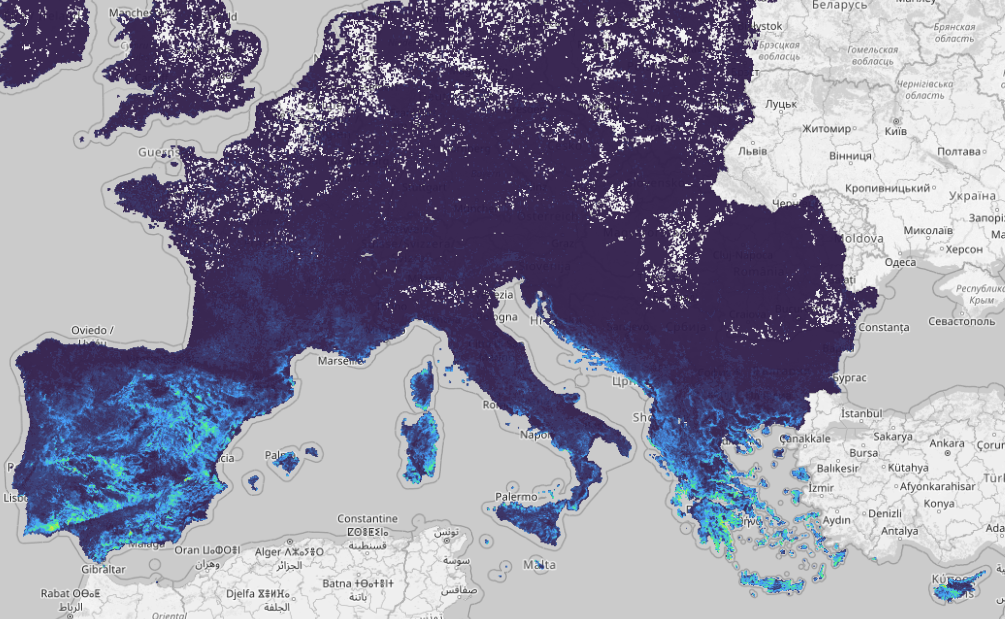
\includegraphics[width=1\linewidth]{figs_06/sclerophyllous.png}
        \caption{Predicted probabilities for Sclerophyllous vegetation.}
        \label{fig:sclerophyllous}
        \end{figure}
        
        The proportional mapping approach demonstrated in Chapter\@~\ref{cha:chapter4} may provide a solution to a discrepancy between given class proportions and mapped hard-class proportions, as long as some level of meaningful probability is predicted in the right locations. In that chapter, we mapped the 8 level 1 LUCAS land cover classes across five years and five countries, and compared the performance of models trained only on the country they mapped with the performance of a model that was trained on data from multiple European countries. We found that proportional maps based on predictions by the general model were of similar accuracy to maps based on probabilities predicted by the less biased local models. This suggests it is possible to train one model that can recognize many classes. If such a model is well-calibrated within each class and the top 5\% of predicted probabilities, for e.g., \textit{Sclerophyllous vegetation}, are indeed the most likely to actually be that class---even if they are overshadowed by more common classes---local area estimates can be used to force them to the forefront in areas where such classes are known to be more numerous. 

        In conclusion, leveraging training data from across a wide temporal and geographical range can strongly improve the accuracy and generalization of land cover classification. Models trained on a diverse temporal dataset consistently outperformed those limited to a single year's data, even when restricted to being trained on similarly sized datasets. Integrating training data in such ways can cause model bias that can strongly reduce accuracy, but these can be countered by incorporating area statistics during the hard-class classification process.
        
    \subsection{How do the number and type of classes in a legend affect the accuracy of land cover classification?}
    \label{syn:rq3}

        In Chapter\@~\ref{cha:chapter3}, we found large differences in hard-class accuracy between the three different levels of the CORINE legend: At level 3, only 10 out of 43 classes were mapped with an F1-score above 0.5 (\textit{Discontinuous urban fabric, Industrial or commercial units, Non-irrigated arable land, Rice fields, Broad-leaved forest, Coniferous forest, Bare rocks, Glaciers and perpetual snow, Peat bogs, and Water bodies}). At level 2, this was 9 out of 14 classes, and at level 1, all 5 classes. At level 3, we can see a positive relationship between the number of samples ('support' in table \ref{tab:cv_accuracy_lvl3}) and the F1-score, although there are classes with many samples that still scored poorly. There are a number of error sources: 

        Firstly, some of these classes are 'mixed types' such as \textit{Complex cultivation patterns}, \textit{Agriculture with significant natural vegetation} and \textit{Mixed forest}. Some other classes occur mostly at a sub-pixel level, in effect being mixed classes with whatever class they border. For instance, \textit{Roads and rail networks and associated land} in Chapter\@~\ref{cha:chapter3}. Stretches of road or rail infrastructure that are wider than 30~m are relatively rare, and this type of land cover is often very close to other classes such as buildings. If there are classes in the same (level of the) legend, these classes 'compete', even if a prediction for any of them would be true. 
        Second, some LULC classes have the same land cover, but differ in land \textbf{use}, such as \textit{Pasture}, \textit{Natural grasslands}, and \textit{Airports} (which also have significant grasslands, see Figure \ref{fig:heathrow_pastures}). Properly distinguishing those classes may require higher temporal and spectral resolution or feature engineering to detect differences in mowing policy or grass species. 

        \subsubsection{The accuracy/detail trade-off}
        
            These mixed class and land use errors largely disappeared when aggregating classes to a level in the hierarchy where mixed nature or land use distinctions ceased to matter, such as \textit{313: Mixed Forests} to \textit{CLC 31: Forests and seminatural areas}. This only works for classes that are placed in a logical order in the legend, for instance, \textit{Pastures} and \textit{Natural grasslands} are considered completely different LULC types even at the highest level of the legend, where they are aggregated to \textit{Agricultural areas} and \textit{Forest and semi-natural areas}, respectively. In the S2GLC legend, however, we both aggregated these grass classes to \textit{Herbaceous vegetation}, which was much more effective. This applied to the S2GLC legend in general: When we summed the probabilities of all classes according to the S2GLC scheme, we achieved similar or higher accuracy than the S2GLC land cover maps. This means that training a model on many classes, even more classes than 'needed' for a specific use case, does not intrinsically harm its accuracy in a simpler legend, even when the land cover predictions are inaccurate at the highest level of detail.

        In conclusion, this thesis proves that the number and type of classes within a land cover classification legend can adversely influence classification accuracy. However, aggregating predictions into a smaller set of less ambiguous classes can negate this impact. Therefore, pursuing the classification of diverse and detailed land cover maps---without the objective of achieving minimum accuracy for each class at the highest level of thematic detail---holds merit.
    
        \begin{figure}[H]
        \centering
        \begin{subfigure}[b]{0.48\textwidth}
        \centering
        \caption{OpenStreetMap}
        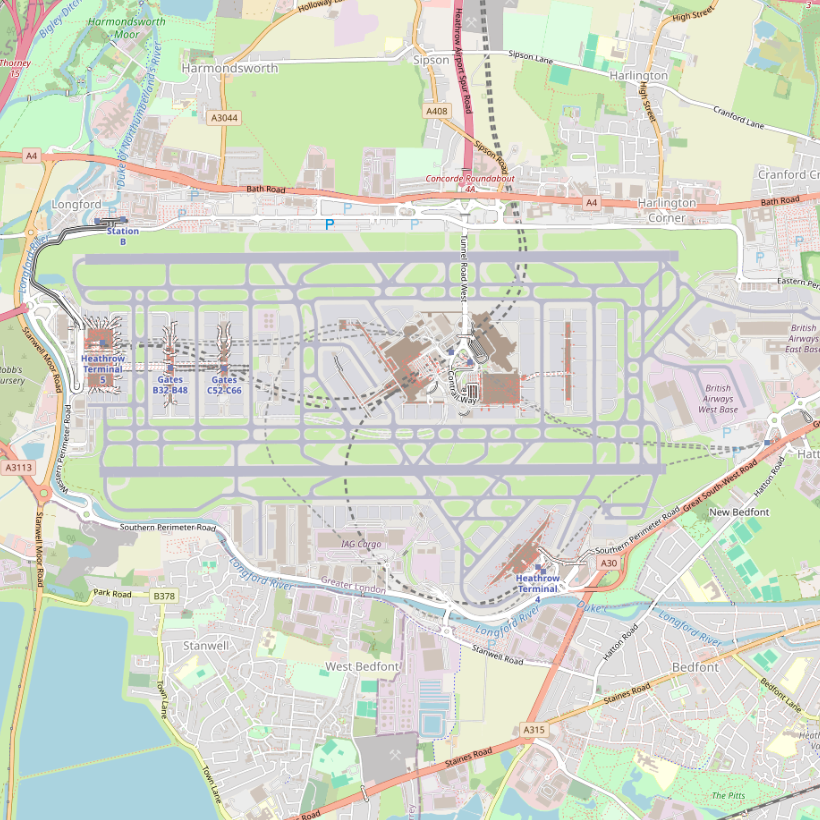
\includegraphics[width=\textwidth,height=0.7\textwidth]{figs_06/heathrow_osm.png}
        \label{fig:heathrow_osm}
        \end{subfigure}
        \hfill
        \begin{subfigure}[b]{0.48\textwidth}
        \centering
        \caption{CORINE Land Cover}
        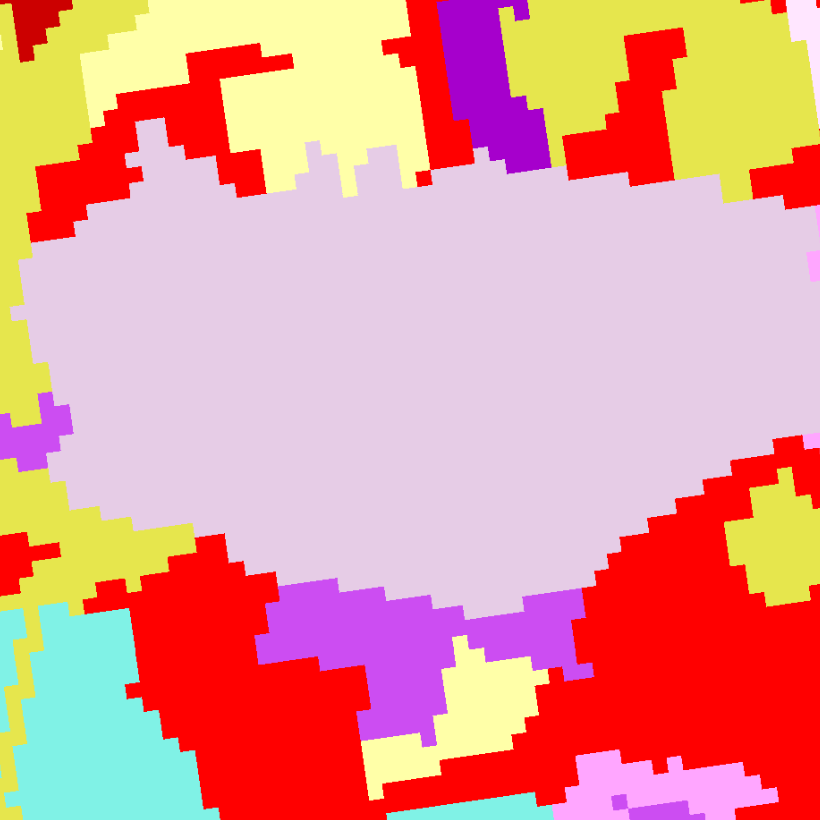
\includegraphics[width=\textwidth,height=0.7\textwidth]{figs_06/heathrow_clc.png}
        \label{fig:heathrow_corine}
        \end{subfigure}
        \vspace{0.5em}
        \begin{subfigure}[b]{0.48\textwidth}
        \centering
        \caption{Probability for \textit{Airports}}
        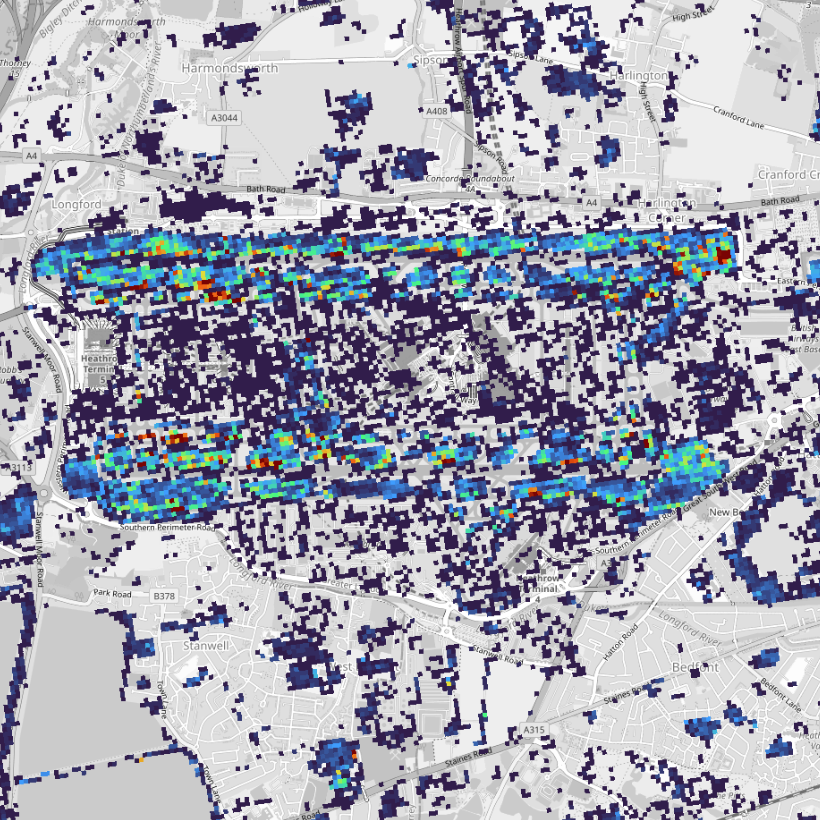
\includegraphics[width=\textwidth,height=0.7\textwidth]{figs_06/heathrow_p_airport.png}
        \label{fig:heathrow_airport}
        \end{subfigure}
        \hfill
        \begin{subfigure}[b]{0.48\textwidth}
        \centering
        \caption{Probability for \textit{Industrial and commercial units}}
        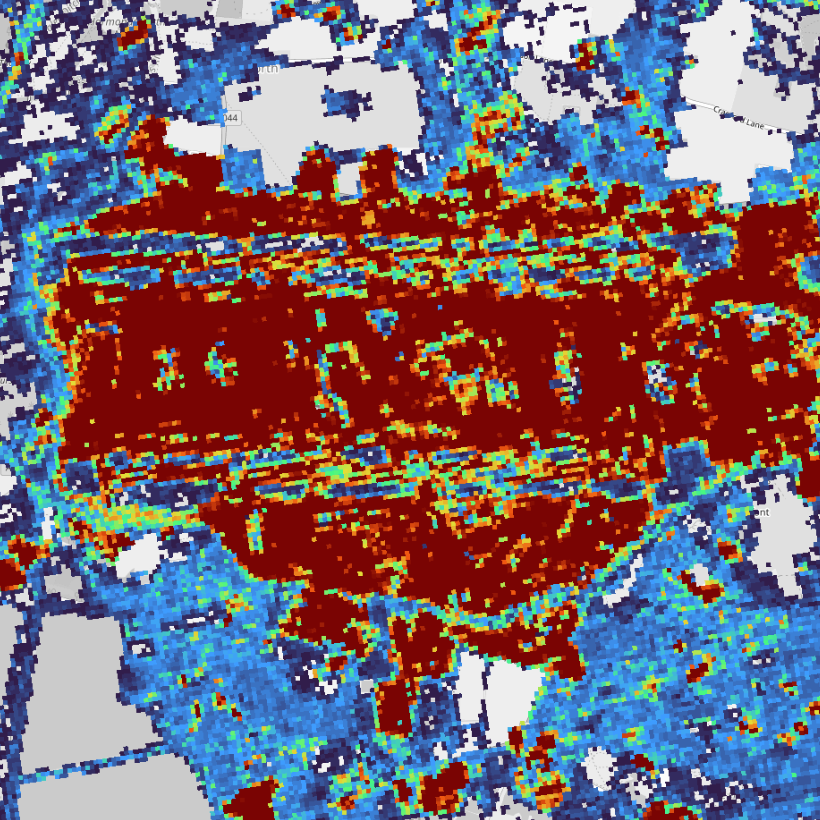
\includegraphics[width=\textwidth,height=0.7\textwidth]{figs_06/heathrow_p_industrial_commercial.png}
        \label{fig:heathrow_industrial-commercial}
        \end{subfigure}
        \vspace{0.5em}
        \begin{subfigure}[b]{0.48\textwidth}
        \centering
        \caption{Probability for \textit{Pastures}}
        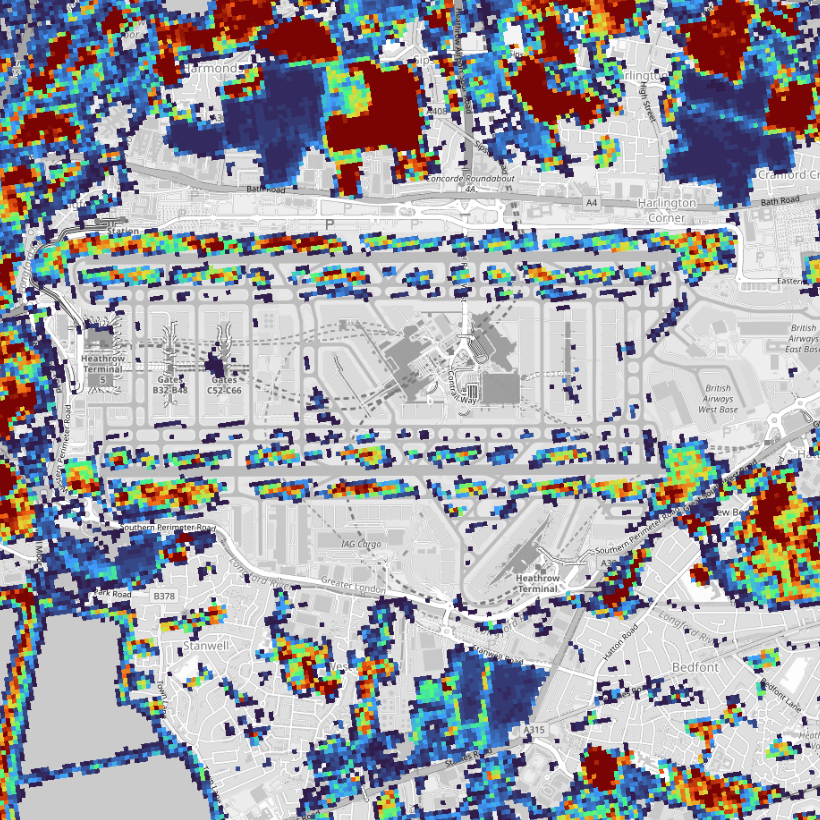
\includegraphics[width=\textwidth,height=0.7\textwidth]{figs_06/heathrow_p_pastures.png}
        \label{fig:heathrow_pastures}
        \end{subfigure}
        \hfill
        \begin{subfigure}[b]{0.48\textwidth}
        \centering
        \caption{Hard-class classification}
        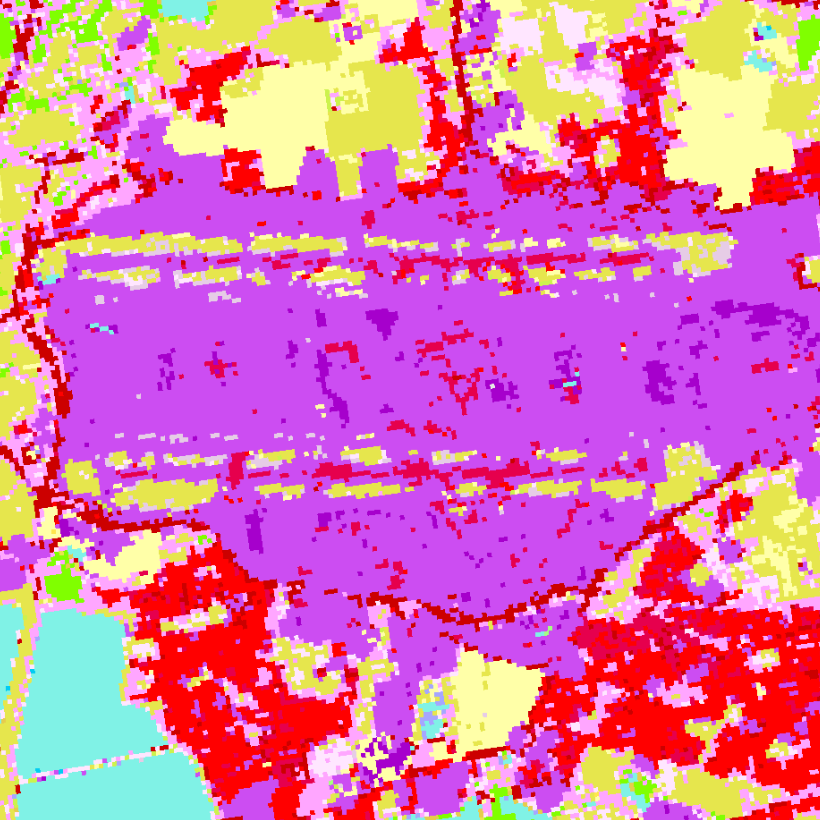
\includegraphics[width=\textwidth,height=0.7\textwidth]{figs_06/heathrow_lulc.png}
        \label{fig:heathrow_industrial-commercial}
        \end{subfigure}
        \label{fig:heathrow}
        \caption{Comparison of CORINE Land Cover and LULC classification from Chapter\@~\ref{cha:chapter3} for Heathrow Airport, London, in 2018. Note that the LULC classification did a decent job classifying the non-residential buildings cultivated grassland that together make up the airport, but failed to assign them to the actual \textit{Airport} class: The purple is \textit{Industrial and commercial units}, while the yellow is \textit{Pastures}, and the red is \textit{Roads}}
        \end{figure}

    \subsection{What is the effect of enforcing correct class proportions on map accuracy?}
    \label{syn:rq4}
 
        In Chapter\@~\ref{cha:chapter4}, we created annual maps of 5 European countries. For each country, we predicted probabilities with a local model that was trained only on data from that country. We also predicted probabilities for each country with a model that was trained on a larger, pan-European dataset. We then made hard-class maps of each country and year in two ways: by maximum probability assignment and with a novel algorithm called Iterative Mapping of Probabilities (IMP).
        
        The IMP algorithm was developed as a tool to produce maps that match existing area estimates without sacrificing accuracy. Our experiments in Chapter\@~\ref{cha:chapter4} show that classifications by IMP tend to be \textit{more accurate} than those by maximum probability assignment, especially in the case of models that are biased to over- and underpredict certain classes. 
        
        Results showed that maximum probability maps using the probability of the local models tended to be more accurate than those by the general model, but this was not the case when using IMP instead of maximum probability assignment. The maps created by IMP were however of equal or better accuracy than those made with maximum probability assignment, while having class proportions as estimated by Eurostat. The effect of IMP on accuracy can be summarized as sacrificing precision (user accuracy) of some classes, to raise recall (producer's accuracy), with a net benefit to higher weighted F1-scores.

        \subsubsection{Future research}
        
        Essentially, IMP quantifies the bias of a model when compared to a given class proportion estimate and uses the iteration probability thresholds to impose its own bias on the model predictions, minimizing the difference between precision and recall.
        While class-wise precision and recall values of proportional maps were closer to each other than those of maximum probability maps, they were not identical. While Eurostat area estimates are considered to be quite reliable, a direct class count from a dataset is by definition 100\% accurate. It is likely that using these counts could further harmonize precision and recall on a class-by-class basis. If this is true, IMP can potentially be used to quantify either how representative a validation dataset is for its study area, or the accuracy of a class proportion (area) estimate. Additional experiments that did not make it into the thesis provide strong suggestions that this is true, and we will keep researching this in the near future.
        
        Chapter\@~\ref{cha:chapter4} showed that IMP provided a greater accuracy improvement to models that were trained on data with a different class distribution than the area they mapped. This means that IMP can be used to optimize the predictions of large land cover models to a regional context without requiring new training or predictions. It also means that IMP can learn the bias of a model if the model is validated in an area for which class proportions can be estimated; the quantification of this bias can then be stored, and used to make proportional maps of areas for which class proportions are not available. This too is a promising line of research that will be continued after this thesis. 

        If reliable and trusted validation data exists for an area, IMP can be used to compare the accuracy of different area estimates by making hard-class maps for each area estimate. The area estimate that matches the reality on the ground most closely should allow IMP to produce the most accurate map. When used this way, IMP could be used to settle disputes about quantities of land cover and land cover change.

        \subsubsection{Wider applicability}
        
        The ability of IMP to quantify and correct model bias extends its usage beyond land cover classification. It can be used for any type of machine learning task where class proportions can be either estimated, targeted, or dictated, and where bias must be quantified. Any field that utilizes machine learning models and faces challenges with class imbalance, representation bias, or requires models to perform accurately across diverse and potentially underrepresented groups could use the algorithm to enhance model fairness, accuracy, and generalization.
        
        For example, in predictive policing and recidivism prediction, biases in the training data can perpetuate and amplify societal biases. Reducing the bias in such models could contribute to fairer decision-making in the criminal justice system \citep{berk2021fairness, dressel2018accuracy}. Financial institutions often use machine learning models for credit scoring and risk assessment. The training data can be biased due to historical decisions and social demographics, potentially leading to unfair assessments. A post-hoc correction algorithm could mitigate these biases, leading to fairer credit scoring and risk assessment models \citep{chen2018why, kamiran2012data}. 

\section{Reflection and outlook}

    This thesis presents a transparent, reproducible framework for combining data from various sources to create detailed, consistent maps. Its chapters show examples of how to combine Earth observation and land cover data from multiple sources, pre-process and harmonize them, and make annual maps with many classes. It shows how to deal with the problems of model bias toward some classes, which may arise when some land cover classes have more data available compared to others.
    
    Combining several datasets from different times and regions to create large and rich training datasets is a challenging task. It requires knowledge of available data sources, technical skills, and extensive spatial, temporal, and thematic harmonization work. This thesis shows that such a dataset can be used to train a model that classifies many classes. While the accuracy at full thematic depth is lacking compared to those of other recent products, we showed that they are of comparable accuracy to similar products when we reduce the number of classes, like CORINE level 1, or include a legend more optimized for remote sensing like S2GLC. We also show that there are benefits to training a model on data from different times, even without performing any kind of time-series analysis. Finally, we show that it is possible to incorporate class proportions such as area estimates into the workflow to create land cover maps that not only match these proportions, but are more accurate than maximum probability maps.

    We have published the code and data that we used and produced in this thesis in the hope that it is useful to other modelers, especially those who are not experts in remote sensing. The analysis-ready feature space and harmonized training datasets can be used by anyone to improve our method and maps. The predicted probabilities of Chapter\@~\ref{cha:chapter3} can be used as input for ensembles to map other types of land cover, potentially much more accurate than the probabilities themselves, just like has been suggested by the creators of DynamicWorld \citep{brown2022dynamic}.

    This thesis not only contributes to the field of remote sensing by enhancing methods for land cover mapping but also sheds light on the role of data integration and methodological innovation in addressing current limitations. Nonetheless, the journey toward comprehensive, dynamic, detailed representation of the Earth's surface is far from complete. As we stand on the threshold of new discoveries and technological frontiers, we are propelled to ask a fundamental question: What is necessary to \textit{map everything, everywhere, all the time}?

    \subsection{Mapping everything: On detailed hierarchical legends}
    \label{syn:everything}

        It is, of course, unfeasible at best to map \textit{everything}. However, there is a clear use case for having detailed and accurate maps that scientists and policy-makers can use for their specific use cases, for example, to distinguish wetland types for bird conservation \citep{fan2021function} or peat bogs \citep{spitzer2006insect} for insect biodiversity. But it extends beyond nature; different categories and qualities of the urban environment are frequently investigated and compared due to their effects on human well-being \citep{krekel2016greener}, socio-economic inequality \citep{tian2024urban}, and large-scale analyses on the sustainability of social-environmental systems \citep{chen2022sustainability}. Especially different vegetation types are becoming increasingly important. Unfortunately, these are also the most variable in space and time, while simultaneously being hard to distinguish, especially on a high thematic resolution. Any class that is mapped needs to be properly represented, both conceptually and in the data. In general, to map LULC at high thematic resolution, we need:
        \begin{enumerate}
        \item A hierarchical legend with meaningful definitions that work for both machines and people;
        \item Training data and area estimates that are compatible with said legend;
        \item A feature space where all classes can be distinguished;
        \end{enumerate}

        \subsubsection{The Stuff of Legends}
        \label{syn:everything-legends}

        In this thesis, I attempted to first (in Chapter\@~\ref{cha:chapter3}) reproduce the CORINE land cover legend, and experienced the limitations of mixed land use / land cover classes, and the contextual overlap between some classes like pastures, industrial buildings, and airports (see Fig\@~\ref{fig:heathrow}). While land use can cause much confusion to some machine learning models, it is essential, perhaps even more so than land cover, to locate and quantify. These limitations can likely be overcome by optimizing the legend and disaggregating land use and land cover in a fine-grained way.
        
        Fortunately, much work has already been done on this. The discussion around the ambiguities of CLC and its incompatibilities to other nomenclatures, like LUCAS, inspired the formation of the Eionet Action Group on Land monitoring in Europe (EAGLE) group, which developed a method to quantify explicit aspects of land cover components (e.g., points, pixels or polygons on a map) that can be combined to assign a meaningful land use / land cover label. The EAGLE system presents a shift from single-class classification of mapped units, and instead characterize them by their land \textbf{cover}, land \textbf{use}, and land \textbf{characteristics} (See Fig.\@~\ref{fig:eagle_structure}). 
        
        \begin{figure}[H]
        \centering
        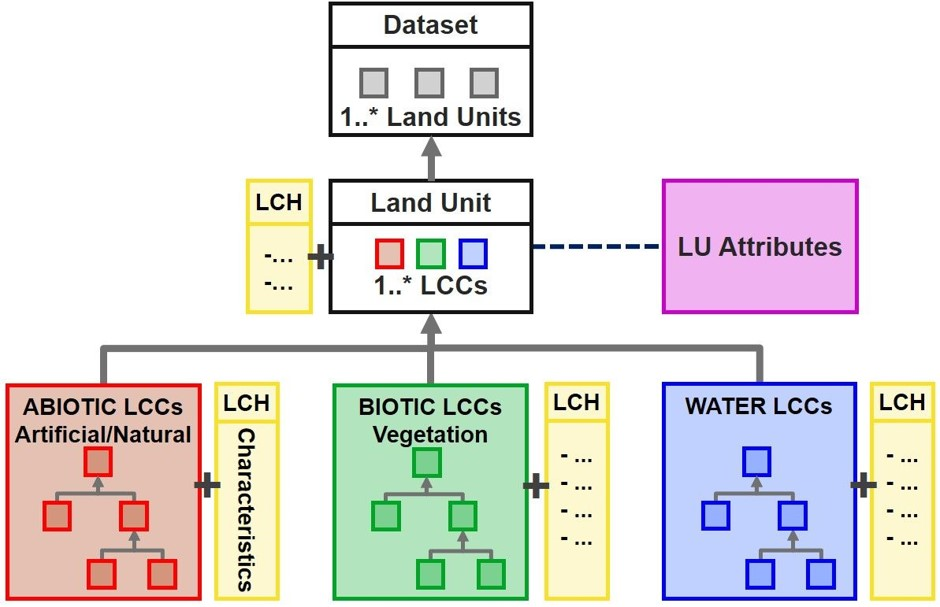
\includegraphics[width=0.75\textwidth]{figs_06/eagle_structure.png}
        \caption{Classification structure of the EAGLE concept: Land Cover (LC), Land Use (LU), and Land Characteristics (LCH) are quantified separately, and can be combined in multiple ways to provide a LULC label to a mapped unit (e.g., a pixel or polygon). Source: \url{https://land.copernicus.eu/en/eagle}}
        \label{fig:eagle_structure}
        \end{figure}
        
        These components are (or consist of) hierarchical legends, and each mapped unit is represented by a combination of these aspects instead of being classified by a single label. For example, \textit{Land Cover} consists of \textit{Abiotic}, \textit{Biotic}, and \textit{Water} land cover categories that each have subtypes (see Figs.\@~\ref{fig:eagle_structure}\@and\@~\ref{fig:eagle_landcover}) such as \textit{Woody} vegetation being split up in \textit{Trees} and \textit{Bushes}. Examples of land \textit{characteristics} are the \textit{frequency of surface water presence through time} \citep{pekel2016high} and \textit{Canopy height} \citep{potapov2021mapping} (See Fig.\@~\ref{fig:eagle_landcharacteristics}). Land \textit{use} is defined at the highest level as the sector of the human economy a piece of land is used for, such as \textit{Primary production}, and then further defined as e.g., \textit{Forestry} and \textit{Agriculture}, in turn, \textit{Agriculture} then contains many different agricultural practices and purposes (See Fig.\@~\ref{fig:eagle_landuse}).
        
        

        \begin{figure}[H]
        \centering
        \begin{subfigure}[b]{0.85\textwidth}
        \centering
        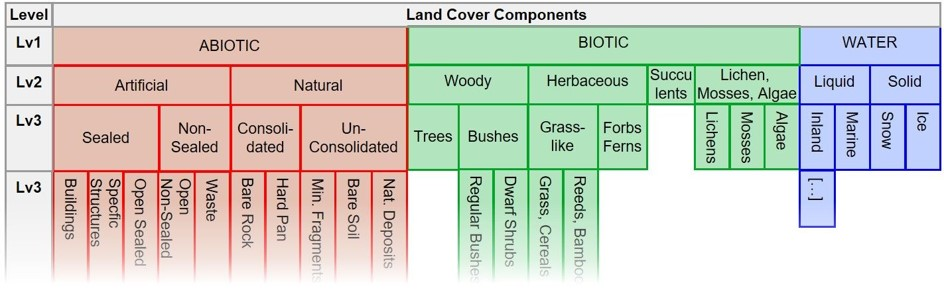
\includegraphics[width=\linewidth,height=0.4\linewidth]{figs_06/eagle_landcover.png}
        \caption{Land Cover Components}
        \label{fig:eagle_landcover}
        \end{subfigure}
        \vspace{1em}
        \begin{subfigure}[b]{0.85\textwidth}
        \centering
        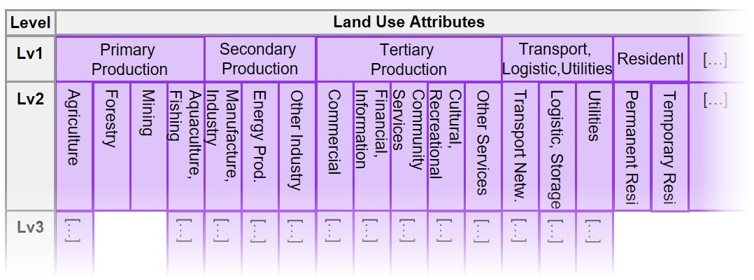
\includegraphics[width=\linewidth,height=0.4\linewidth]{figs_06/eagle_landuse.png}
        \caption{Land Use Attributes}
        \label{fig:eagle_landuse}
        \end{subfigure}
        \vspace{1em}
        \begin{subfigure}[b]{0.85\textwidth}
        \centering
        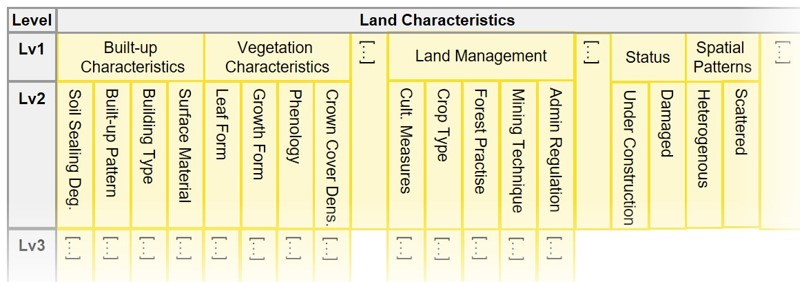
\includegraphics[width=\linewidth,height=0.4\linewidth]{figs_06/eagle_landcharacteristics.png}
        \caption{Land Characteristics}
        \label{fig:eagle_landcharacteristics}
        \end{subfigure}
        
        \caption{A simplified representation of the EAGLE concept and how it can be used to divide land units into categories based on hierarchical combinations of land cover, land use, and water presence. Source: \url{https://land.copernicus.eu/en/eagle}}
        \label{fig:eagle} % This should be inside the figure environment but outside any subfigure
        \end{figure}

        I have shown that aggregating predictions to simpler and/or more optimal legends can drastically improve their accuracy. It would not be surprising if the greater confusion at higher thematic detail has motivated other attempts to create CORINE land use / land cover predictions to pre-emptively reduce their level of detail. But what if you could selectively reduce the detail of predictions that are probably mistakes? 
        
        Using prediction uncertainty to allow a model to predict \textit{nothing} is called \textit{Selective classification}, but this would cause gaps in a map. While no one wants mistakes on their map, why would you throw out the baby with the bathwater to get rid of them? 
        
        A well-designed hierarchy can be used to \textit{save the baby} in the case of uncertain predictions at high thematic detail. For example, it may be hard to correctly distinguish the class of a mixed \textit{Wheat} and \textit{Grass} pixel if it's on the edge of a field, or at the start of the growing season. Prediction uncertainty metrics could be used to aggregate such pixels to a sensible common class, such as \textit{Herbaceous vegetation}. The prediction would then 1) be correct instead of incorrect, 2) be useful instead of empty and 3) indicate prediction uncertainty in a way that humans can easily comprehend.

        Doing this requires a reliable way to quantify prediction uncertainty, in the explicit sense of \textit{``the probability that this specific pixel is a misclassification''}. Our first attempt, the \textit{``model deviance''} from Chapter\@~\ref{cha:chapter3}, is calculated by taking the standard deviation of predicted probabilities by each learner in an ensemble. While we found no significant relationship to the chance that a given pixel prediction is correct, it turned out to be a useful proxy for indicating the distance from the nearest training point of a given class in the feature space. However, there are several metrics that have a stronger theoretical foundation to quantify prediction uncertainty. The most straight-forward and often-used is the highest probability among predicted probabilities. This metric is only reliable when the model is well-calibrated \citep{niculescu2005predicting}, because models can also be ``confidently incorrect''. \citet{calderon2021high} and \citet{bonannella2023biomes} used the \textit{margin of victory}, which is a useful metric for how confident the model is between classes. Conformal prediction promises statistical guarantees of correct error estimation \citep{angelopoulos2023predictionpowered} and is recently finding traction in the land cover community \citep{valle2023quantifying, singh2024uncertainty}. Finally, in Chapter\@~\ref{cha:chapter4}, we found indications that there is a robust relationship between the iteration at which a pixel is classified, and how likely it is to be correct. 

        \subsubsection{Training Data Montage}
        \label{syn:everything-trainingdata}

            No single training dataset currently contains all classes that can be mapped. For example, not even detailed legends like LUCAS have unambiguous exclusive labels for increasingly important objects such as solar panels. To make internally consistent maps with a unified approach, it is therefore essential that existing and future open LULC-annotated data can be integrated in a modular and flexible way, especially without 1) adverse effects from class imbalance in the resulting dataset and 2) sacrificing detail from aggressive legend harmonization.
            
            The effect of class imbalance from dataset concatenation can be countered by applying IMP or similar processes that adjust for model bias. The ability of IMP to correct the bias of a model post-hoc means that models don't need to be trained on datasets that respect class balance, like other mapping \citep{waldner2016towards,kleinewillinghofer2022unbiased}, as long as accurate area estimates are available. This means it can be combined with automated training data generation techniques that don't respect class distributions, such as extracting points from polygons \textit{en masse}, as was done in this thesis. It also means that training datasets with different distributions and classes can be easily combined.
    
            Using a disaggregated set of land cover and land use legends, in line with the EAGLE concept, will allow us to more easily combine existing training datasets. Because different biotic, abiotic, and water land cover classes, as well as land use classes, can simultaneously be present on a pixel, a multi-label classification system would be a logical choice \citep{sumbul2020deep}. Any actual LULC class in the legend can then be calculated by summing the probabilities of all labels that contribute to it. This can even work for different levels of a hierarchical legend \citep{wehrmann2018hierarchical}. Multiple predicted labels from different levels in a hierarchical legend can be combined to represent a single meaningful class. For example, two land cover classes \textit{Herbaceous vegetation}, \textit{Grass} and two land use classes \textit{Primary production} and \textit{Grazing} can be combined to represent 'pasture'.

        \subsubsection{Featuring: Space}

            However, regardless of how meaningful, effective, and detailed its legend, a LULC map can only be as good as the data used to detect them. 
            
            In this thesis, we primarily used a temporally aggregated version of the long-running Landsat archives due to its objective to make consistent time-series of maps and to enable the use of training data from legacy datasets such as CORINE. While the Landsat archives provide a consistent dataset spanning decades, its relatively low spatial, spectral, and temporal resolution limited the classification accuracy of several classes. 
            
            For example, different vegetation types are often best distinguished based on their profile in the electromagnetic spectrum \citep{xu2021towards,hennessy2020hyperspectral, neinavaz2021thermal}. Furthermore, crop types, in particular, benefit from high temporal resolution \citep{esch2014differentiation,xu2021towards}. Their growth cycles, during which their appearance and spectral profile changes drastically, combined with temporal dynamics such as crop rotation, fallow periods, and other practices, require a high frequency of EO data. Making use of Sentinel-2 imagery, with its revisit time of 10 days and higher spatial resolution (10~m), would have limited the time range of the maps to 2015 but might improve performance, as suggested in Chapter\@~\ref{cha:chapter2}. If the emphasis is on mapping longer time series, the framework could be significantly improved by incorporating the NASA Harmonized Landsat and Sentinel-2 (HLS), which combines the longevity of the Landsat program with the high temporal resolution of the Sentinel program \citep{claverie2018harmonized}.
            
            In the longer term, Landsat Next, scheduled to start providing data in 2030, promises substantial improvements while ensuring compatibility with both its own predecessors and other systems (See Fig.\@~\ref{fig:landsat_next}. The 26 spectral bands of this new iteration will match the 11 'heritage' bands of previous Landsat programs but will also contain 5 bands with similar spatial and spectral characteristics as Sentinel-2, improving revisit time from 16 to 6 days \citep{landsatnext2023}. Similarly, ESA's Copernicus Hyperspectral Imaging Mission for the Environment (CHIME) will have over 200 spectral bands and a revisit time of 12.5 days, revolutionizing hyperspectral Earth observation \citep{nieke2023copernicus}. Meanwhile, the German Aerospace Center's recently launched Environmental Mapping and Analysis Program (EnMAP) system, with 228 hyperspectral bands and a revisit time of only 4 days, is particularly suitable for distinguishing vegetation types such as crops and tree species. It is already available and being used to map LULC, showcasing the utility of high spectral and temporal resolution in current remote sensing applications \citep{storch2023enmap, lekka2024appraisal}.
    
            \begin{figure}
            \centering
            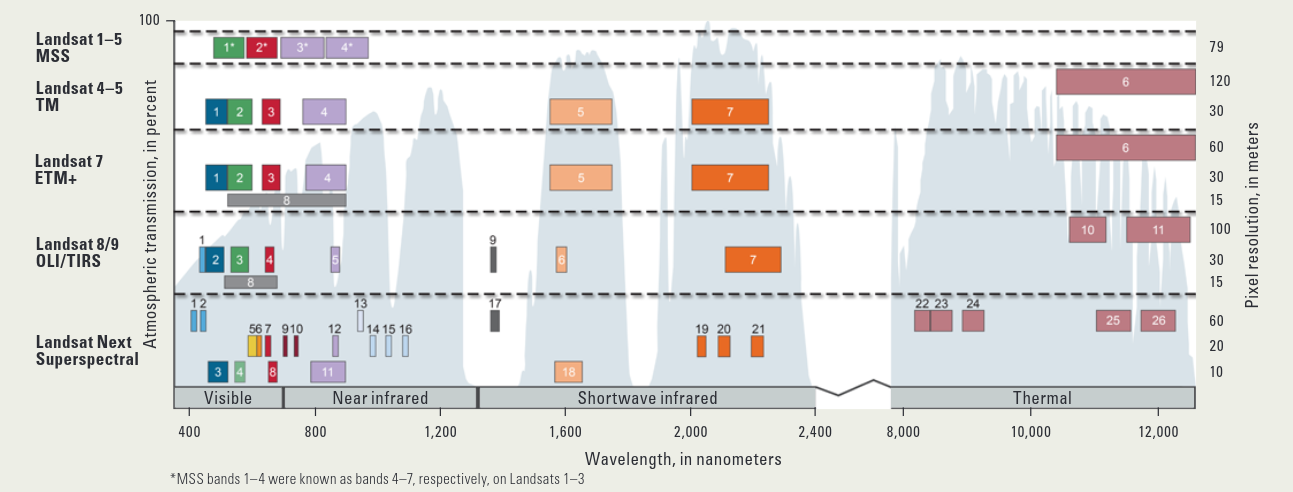
\includegraphics[width=1\linewidth]{figs_06/landsat_next.png}
            \caption{Comparison of pixel resolution and spectral bands between Landsat Next and previous Landsat satellites. From: \citep{USGS2024LandsatNext}}
            \label{fig:landsat_next}
            \end{figure}
        
    \subsection{Mapping everywhere: Moving beyond Europe}
    \label{syn:everywhere}

        The framework presented in this thesis relies on openly available land cover samples for training and validation, and benefits greatly from accurate area estimates. Thanks to the efforts of European institutions, such as Eurostat, the EEA and JRC, such resources exist for Europe. Its high levels of collaboration, organization and prosperity also facilitate other projects that can be good sources of training data, such as the impressive EUBUCCO \citep{milojevic2023eubucco} building dataset.
        
        Most other continents, however, are not similarly fortunate. For example, the LUCAS land cover observations \citep{dandrimont2020harmonised} have allowed many global maps to be validated and compared in Europe \citep{gao2020consistency,venter2022global}, but this is more difficult to do in a standardized way in countries and continents that have a less detailed, reliable, or otherwise representative validation dataset.

        Furthermore, land cover and land use represent the diverse ways humans interact with the environment, influenced by geographical, cultural, and economic factors that vary widely across regions. To extend the proposed framework to other continents and make global maps at high thematic detail, such differences need to be acknowledged and accounted for. To do this, we need global samples and statistics, and supplement them with data that is meaningful on a local scale.

        \subsubsection{Global differences}
        
            A global map needs to reflect the significant differences between land cover and land use types across various regions. These differences stem from diverse administrative norms, capacities, environmental contexts, and land use needs. 
            
            For instance, the classification systems and the types of crops that are prevalent in different biomes vary widely. In Europe, the distinction between crops is typically made in July to capture peak growing seasons \citep{esch2014differentiation,xu2021towards}, whereas the monsoon cycle determines India's Kharif (June--October) and Rabi (November--April) seasons.
            Projects like WorldCereal address these challenges by creating a collection of regional maps, each tailored to the unique agricultural seasons of the area it represents \citep{tricht2023worldcereal}.
            
        \subsubsection{Global data}
            \label{syn:everywhere-globaldata}

            To map relevant LULC classes globally (or at least in other continents than Europe), training and validation data from those areas is needed. For this purpose, we can combine generic global training datasets like the Dynamic World training data \citep{tait2021dwtd} and GLANCE \citep{stanimirova2023global} with global datasets that represent a few detailed classes such as WorldCereal \citep{boogaard2023worldcereal} and NASA CropHarvest \citep{tseng2021cropharvest}. 
            
            Volunteered geographical data is another important source of detailed class labels. For example, OpenStreetmap was used to extract training data and map 14 CORINE classes more accurately than CORINE Land Cover in most cases \citep{schultz2017open}. In 2016 OSM's road network was 83\% complete, and more than 40\% of countries, including several in the developing world, had a fully mapped street network \citep{barrington2017world}. Still, its coverage for other objects is far from perfect, as even in Europe, the extent to which buildings and other objects are annotated is heavily biased to areas that are more prosperous or more popular with prosperous tourists (See Fig.\@~\ref{fig:osm_vs_cop_italy}

            \begin{figure}
            \begin{subfigure}[t]{0.33\textwidth}
            \centering
            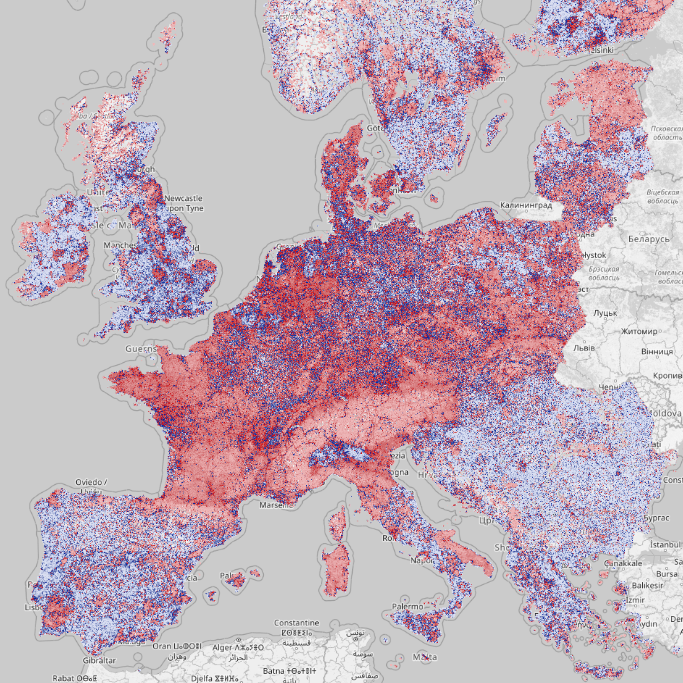
\includegraphics[width=\linewidth,height=\linewidth]{figs_06/osm_impcop.png}
            \caption{Europe}
            \label{fig:osm_vs_cop_europe}
            \end{subfigure}
            \hfill
            \begin{subfigure}[t]{0.66\textwidth}
            \centering
            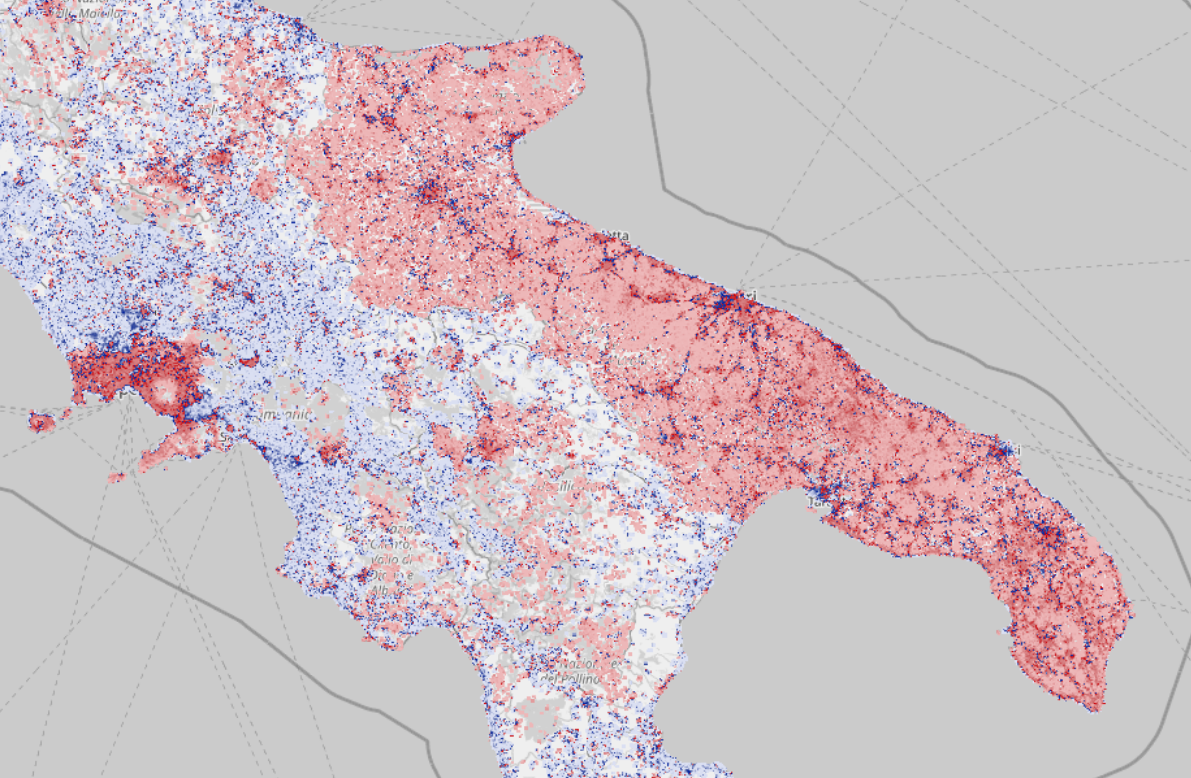
\includegraphics[width=\linewidth,height=0.5\linewidth]{figs_06/osm_vs_cop_italy.png}
            \caption{Southern Italy}
            \label{fig:osm_vs_cop_italy}
            \end{subfigure}
            \caption{extracted OpenStreetMap buildings (in red), supplemented by Copernicus High Resolution Imperviousness data (in blue), used in Chapter\@~\ref{cha:chapter3}. The red areas indicate where buildings are annotated in OSM, while blue indicates impervious areas that are most likely buildings, but were missed by OSM. It shows clear differences between country borders (e.g., between France and Spain, Austria and Slovenia), regions (e.g., Puglia and Campagna in Southern Italy), and the urban/rural divide. For a more detailed explanation of this dataset, see Chapter\@~\ref{cha:chapter3}.}
            \label{fig:osm_vs_cop_europe}
            \end{figure}
            
            The detail of such a global dataset can then be enriched with localized datasets that represent the landscape of different regions in locally relevant classes, such as CATLC \citep{garcia2022catlc}. In Section\@~\ref{syn:everything-trainingdata}, we already suggest ways that a combination of multi-label classification and IMP can be used to combine diverse datasets with incompatible legends and class balances. In this context, it would mean that a model analyzing a dense sclerophyllous forest in the Mediterranean can predict \textit{Forest} based on DynamicWorld training data \citep{tait2021dwtd}, \textit{Dense Forest of sclerophylls} based on data from CatLC \citep{garcia2022catlc}, and\textit{Sclerophyllic vegetation} from Corine Land Cover and S2GLC \citep{jenerowicz2021validation}. 

            To effectively combine polygon and point data sources, a point sampling technique such as the one used in this thesis can be applied, creating a harmonious point dataset. Although this limits the number of modeling techniques, especially more modern ones such as convolutional neural networks, interesting work has been done on \textit{weakly supervised image classification} \citep{huang2018weaklysupervised}. This technique allows powerful deep learning image segmentation models to be trained without fully annotated pixel maps, instead only requiring labels about the classes that are present \textit{somewhere in the image} (See Fig.\@~\ref{fig:weaklysupervised}. Applying this technique to land cover classification would ameliorate the need for costly wall-to-wall annotations that are currently used in many benchmark datasets such as CatLC \citep{garcia2022catlc} and BigEarthNet \citep{sumbul2021bigearthnet}, and would improve the value of legacy and novel point-wise observations such as LUCAS \citep{dandrimont2021lucas} and GeoWiki \citep{fritz2012geo}.

            \begin{figure}[H]
            \centering
            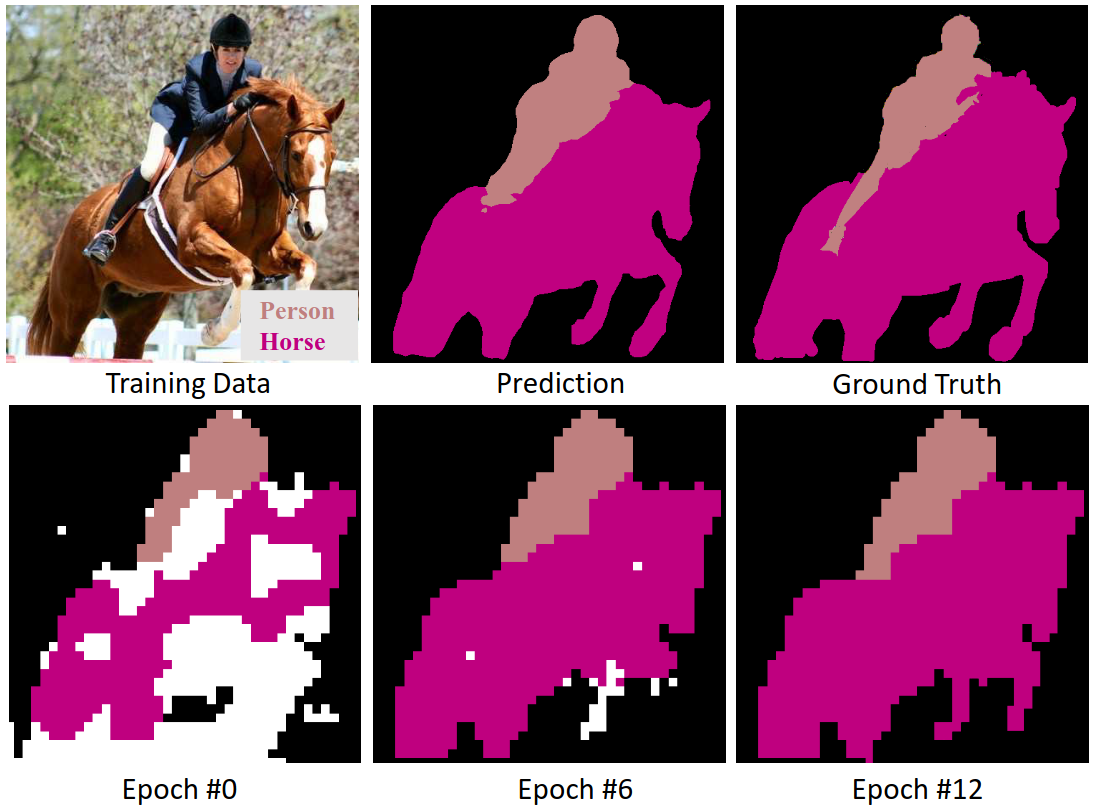
\includegraphics[width=0.5\linewidth]{figs_06/huang_person_horse.png}
            \caption{Example of the training process of a weakly supervised semantic segmentation model, from \citet{huang2018weaklysupervised}. The top row shows a training image that is only annotated with the classes that are present in the image, as well as the predicted and true class membership of each pixel. The bottom row shows the performance of the model at various steps (epochs) in the training process.}
            \label{fig:weaklysupervised}
            \end{figure}

        \subsubsection{Global statistics}

        It is imperative to counter the effects of class imbalance that can be caused by combining different datasets, or by using data from a large region (See Chapter\@~\ref{cha:chapter3} and Section\@~\ref{syn:rq2}). In Chapter\@~\ref{cha:chapter4}, we have shown that this is possible by using area statistics from official sources. This is not a novel concept: \citet{you2014generating} used multiple datasets, including area statistics from governmental organizations, to map the area of twenty different crop types. What is novel, however, is that IMP might be generalizable through space and time, when the predictions are made in a consistent feature space.

        IMP offers a promising way to address class imbalance and model bias in land cover classification, even when detailed area statistics are not universally available. The algorithm tackles model bias by analyzing cut-off probability values for each class across iterations. The key idea lies in generalizability: if the confusion patterns between classes are similar across regions, IMP might be applicable even without area estimates. You could store the probability threshold for each class at each iteration and apply them to probabilities predicted by the same model for a different area. This can be explored in a European context by mapping neighboring NUTS2 areas of the ones we have already mapped, using the cutoff values of their originally mapped neighbor. We can then 'pixel count', and compare the counts to the area estimates. This could make the method applicable for areas that are less meticulously quantified than Europe. This will still require area estimations to be done in some representative locations, but does not require continent- or country-wide surveys. 
        
    \subsection{Mapping all the time: Temporal resolution and range}
        \label{syn:allthetime}

        Approaches that map many things will need a rich feature space and will likely not be useful for rapid detection of, for example, illegal deforestation or natural disasters. 

        \subsubsection{Long-term analysis}
        They will be useful for assessing long-term trends though. In Chapter\@~\ref{cha:chapter3}, we used regression on the predicted probability time-series per pixel to analyze the long-term trends predicted by our model (See Fig.\@~\ref{fig:brocken_slope_analysis}). While the method we used had problems with extremely negative slopes being quantified as 'no data' (see Fig.\@~\ref{fig:brocken_pslope}), the slope of the harmonized NDVI trend (Fig.\@~\ref{fig:brocken_ndvi}) and annual predicted probabilities for \textit{Coniferous forests} accurately shows the mass dieback of Norway spruce trees following a bark beetle infestation in the area \citep{meyer2017matter}.

        More sophisticated and robust pixel-wise trend analysis techniques can be used to quantify gradual processes, like competition and succession of different plant species, which is becoming more relevant in the light of global climate change \citep{bonannella2023biomes}. Having long-term, well-calibrated predicted probabilities for many classes, based on a rich, harmonized feature space, would allow many different users to conduct their own analysis on the classes that are relevant to their use case, such as drivers of deforestation \citep{masolele2024mapping} or mapping and assessing wetlands ecosystem services \citep{fitoka2020water}. In this light, there is a unique value to primarily relying on long-running datasets with a high likelihood of future continuity, such as the Landsat program.
        
        \begin{figure}[H]
        \centering
        \begin{subfigure}[t]{0.24\textwidth}
        \centering
        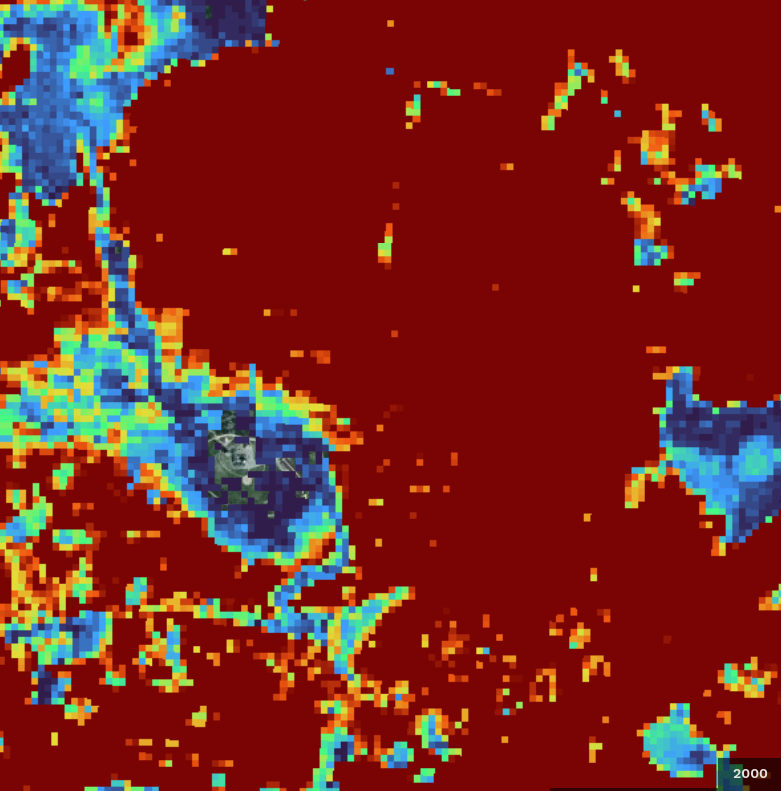
\includegraphics[width=\linewidth,height=\linewidth]{figs_06/brocken_2000.png}
        \caption{2000}
        \end{subfigure}
        \hfill
        \begin{subfigure}[t]{0.24\textwidth}
        \centering
        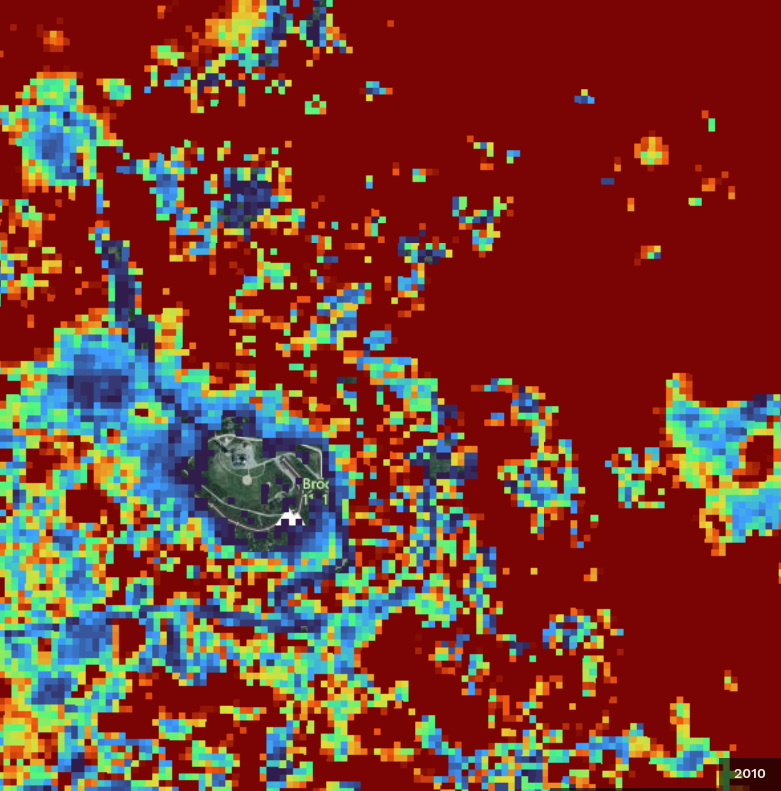
\includegraphics[width=\linewidth,height=\linewidth]{figs_06/brocken_2010.png}
        \caption{2010}
        \end{subfigure}
        \hfill
        \begin{subfigure}[t]{0.24\textwidth}
        \centering
        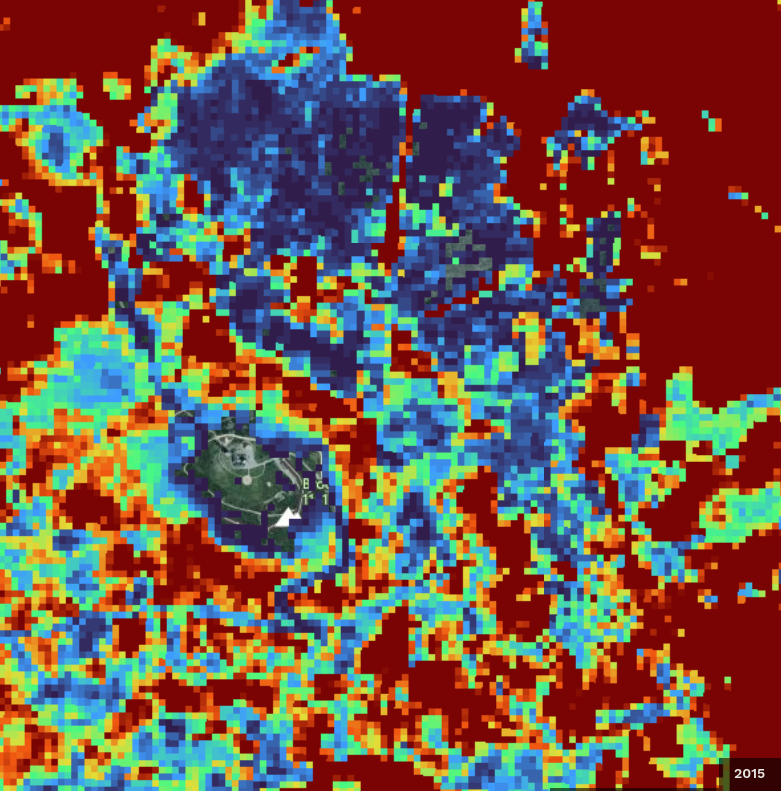
\includegraphics[width=\linewidth,height=\linewidth]{figs_06/brocken_2015.png}
        \caption{2015}
        \end{subfigure}
        \hfill
        \begin{subfigure}[t]{0.24\textwidth}
        \centering
        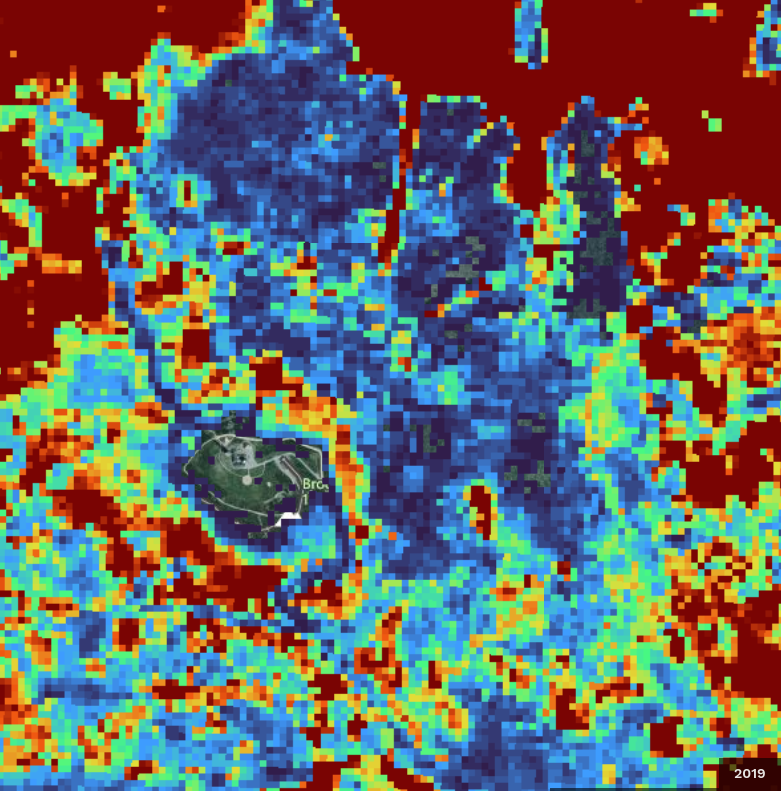
\includegraphics[width=\linewidth,height=\linewidth]{figs_06/brocken_2019.png}
        \caption{2019}
        \end{subfigure}
        \hfill
        \caption{Predicted probabilities for coniferous forest (Norway spruce) near Mt. Brocken, Germany in four years. Blue indicates low probabilities, red indicates high probabilities.}
        \label{fig:brocken_probabilities}
        \end{figure}

        \begin{figure}[H]
        \centering
        \begin{subfigure}[t]{0.24\textwidth}
        \centering
        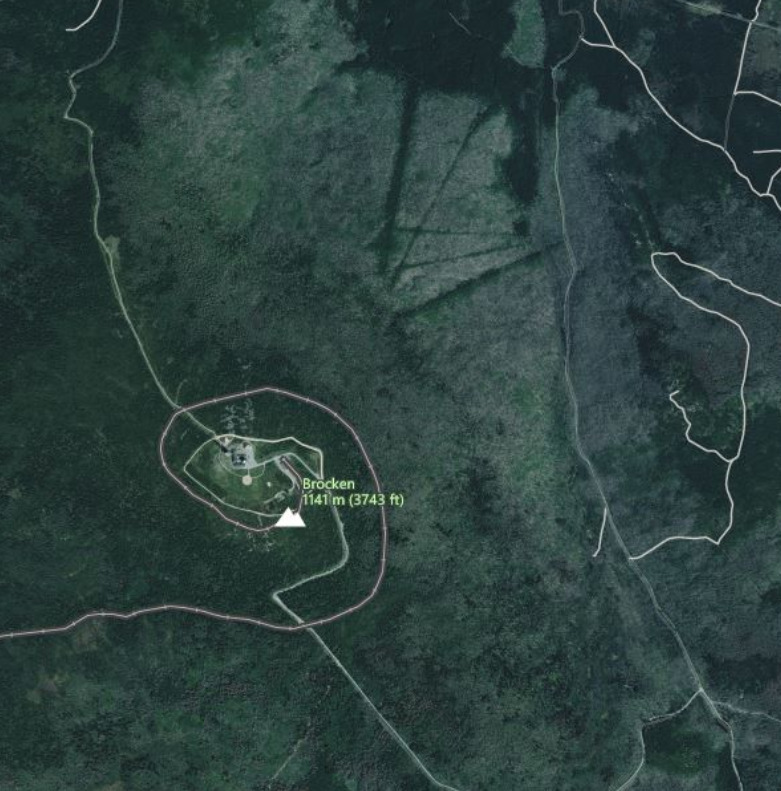
\includegraphics[width=\linewidth,height=\linewidth]{figs_06/brocken_bing.png}
        \caption{High-resolution imagery of the east side of Mt. Brocken. Source: Microsoft Bing}
        \end{subfigure}
        \hfill
        \begin{subfigure}[t]{0.24\textwidth}
        \centering
        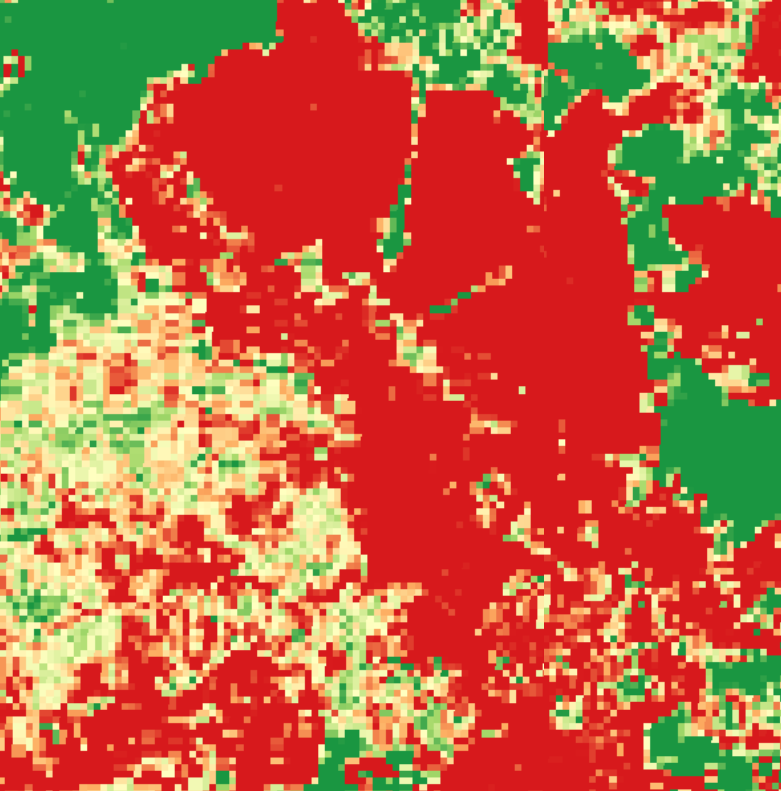
\includegraphics[width=\linewidth,height=\linewidth]{figs_06/brocken_ndvi_slope.png}
        \caption{20-year trend slope of Landsat NDVI values.}
        \label{fig:brocken_ndvi}
        \end{subfigure}
        \hfill
        \begin{subfigure}[t]{0.24\textwidth}
        \centering
        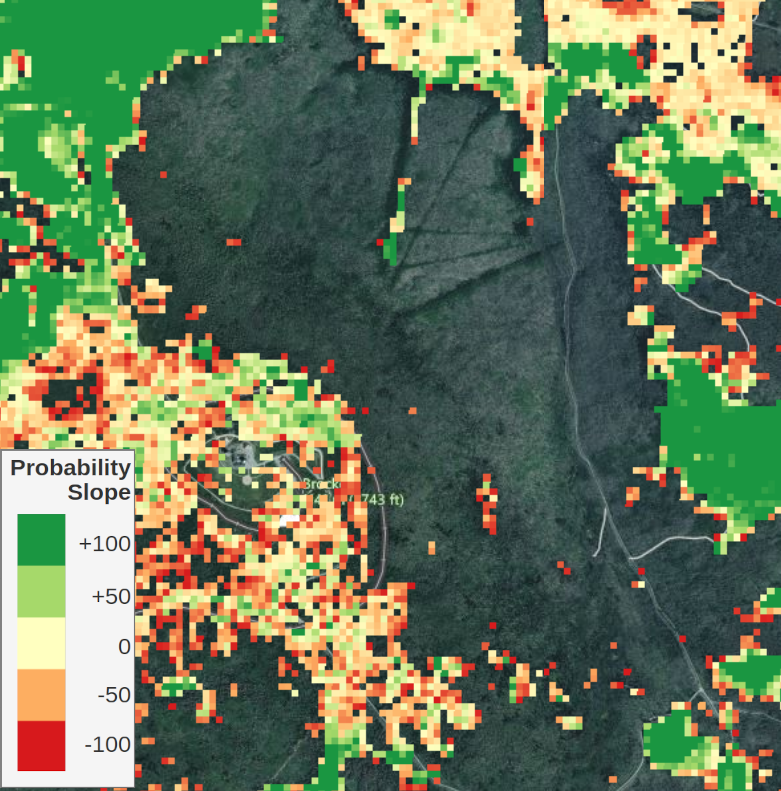
\includegraphics[width=\linewidth,height=\linewidth]{figs_06/brocken_pslope.png}
        \caption{Probability slope for \textit{Coniferous forest}.}
        \label{fig:brocken_pslope}
        \end{subfigure}
        \hfill
        \begin{subfigure}[t]{0.24\textwidth}
        \centering
        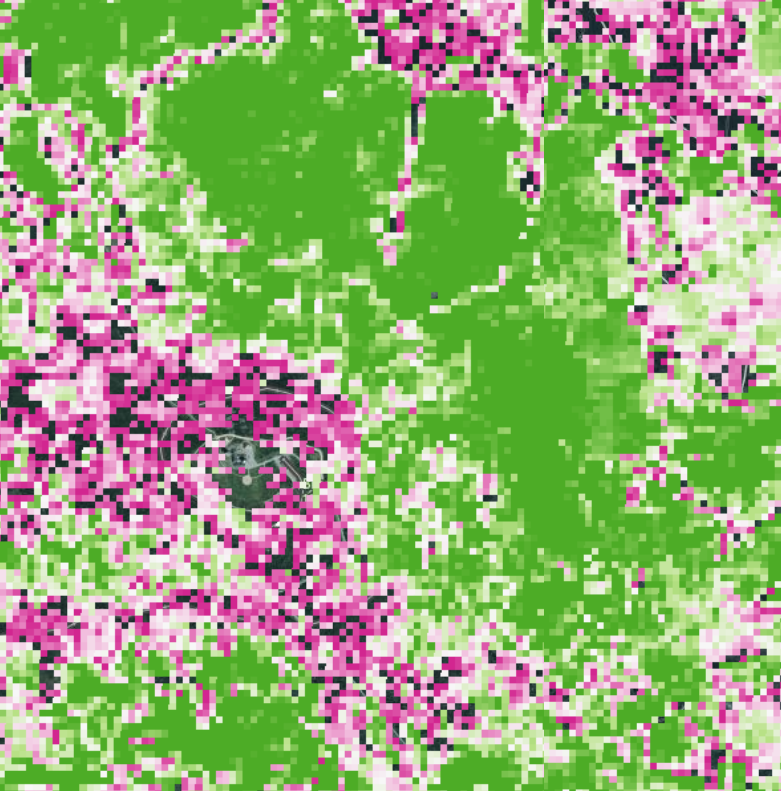
\includegraphics[width=\linewidth,height=\linewidth]{figs_06/brocken_pslope_r2.png}
        \caption{R2 of probability slope for \textit{Coniferous Forest}.}
        \label{fig:brocken_pslope_r2}
        \end{subfigure}
        \caption{Dieback of coniferous forest (Norway spruce) near Mt. Brocken, Germany, as represented by data generated in Chapters\@~\ref{cha:chapter2}\@~and\@~\ref{cha:chapter3}. Note that the \textit{``Probability Slope''} has nodata exactly where it should be highly negative and has a high confidence, but that the \textit{``NDVI slope''} correctly displays the area where the dieback occurred.}
        \label{fig:brocken_slope_analysis}
        \end{figure}

        \subsubsection{Temporal resolution}

        Creating long-term land cover maps that capture temporal dynamics is a complex task. While annual maps seem intuitive, they struggle to represent the changing nature of land cover classes like crops, which undergo various phenological stages \citep{russwurm2023end}, fallow periods \citep{tong2020forgotten}, and other transitions \citep{rodriguez2024classification} throughout the year. The "right" long-term map period depends on the specific application and the land cover classes of interest. 
        
        However, to help work with time periods of six months or more, one possible approach involves using multi-temporal classes in the legend system. These classes could represent sequential land cover types within a single year. For example, \emph{``Cotton-Wheat''} could indicate an area planted with cotton followed by wheat in the same year. By incorporating this strategy, annual or seasonal maps can still be informative. These maps would depict the dominant land cover for a specific period while acknowledging the sequential changes that occur throughout the year. This approach provides a balance between detail and usability, without overwhelming users with excessive maps.
                
        Increasing the temporal resolution to capture frequent changes comes with trade-offs. Highly detailed maps (e.g., daily or weekly) can become computationally expensive. For time-series methods that require observing the entire land cover cycle, a time period with a time resolution that captures the full cycle is crucial. Many crops have cycles lasting 3-4 months, suggesting that bi-weekly or monthly resolutions might be more suitable for these cases. Evergreen broadleaf forests face much less changes along the entire year. In this case, monthly or bi-monthly resolution might be more appropriate. This allows the model to "see" the complete transformation of the land cover throughout the season or the year and improve classification accuracy. 

    \subsection{Mapping it all at once? A final word on models}

        In each of the previous sections about classes and legends (\ref{syn:everything}), training data and feature space (\ref{syn:everywhere}), and the role temporal resolution and coverage (\ref{syn:allthetime}), I have only briefly mentioned modeling techniques that would be appropriate to deal with their specific issues. While each separate question has separate answers, the modeling part of this synthesis must be answered holistically. This final section presents my perspectives on a modeling approach to make detailed, global maps that have useful and meaningful LULC classes. 
        
        I have previously mentioned that different models and feature spaces are optimal for different types of land cover, that global mapping would benefit from an adaptable weakly supervised system that can combine the diverse offer of open datasets, and that the type of classes is intrinsically linked to the temporal resolution of the mapping approach, especially when going beyond mapping land \textit{cover} only.

        A modeling approach is needed that:
        \begin{enumerate}
            \item Classifies many different LULC classes by incorporating:
            \begin{enumerate}
                \item Spatial context (e.g., for airports and urban green);
                \item Temporal dynamics (e.g., for agricultural practices and flood plains)
            \end{enumerate}
            \item Can be understood and trusted by scientists and policy-makers;
            \item Can be trained on mixed point data with diverse overlapping legends;
            \item Can deal with potentially imbalanced training dataset.
        \end{enumerate}

        That is why I propose, and hope to contribute to, the following approach:

        \subsubsection{Hierarchical Multi-label Classification for Legendary Learning}
            The LULC legend should have many different classes in a single hierarchical legend with many levels. The model should be trained with a loss function that varies its penalty based on where errors happen in the hierarchy: For example, errors between tree species should be penalized less harshly than errors between buildings and trees. Previous work on constraining predictions to correct hierarchy paths exists and is called \textit{Hierarchical multi-label classification} \citep{wehrmann2018hierarchical}.

        \subsubsection{Pixel-based uncertainty estimates}
            The final output of the model must have pixel-based uncertainty estimates so that subsequent modeling and decision-making can properly weigh the risks and rewards of using the data.

            An additional benefit of having a robust uncertainty metric is that likely errors in the LULC classification can be aggregated to higher levels in the hierarchical legend. This requires the legend to be designed in such a way that confusion between similar classes is minimized by ascending to higher levels. This can be done in two ways. The first method is a top-down, human-assumed way like EAGLE, where splits happen on a conceptual basis between biotic and abiotic at the top, and between different species of the same vegetation types at the bottom of the legend. The second method is by analyzing the confusion matrix of initial predictions, and forming the aggregation decision tree purely based on which classes are more likely confused by the model. The first method has the advantage of being more interpretable by humans, while the second method has the advantage of likely being more effective at minimizing error by reducing detail. In either case, pixel-based prediction uncertainty must be derived using a robust metric (See section\@~\ref{syn:everything-legends}.

        \subsubsection{An Interpretable Land Cover and Characteristic Ensemble}
            Several models are trained to classify land cover types, such as water and herbaceous vegetation, and land characteristics such as height and photosynthetic activity. These models are trained on point samples on a diverse, modular set of training data to make monthly predictions on a pixel-by-pixel basis. For some classes, especially crops, it is essential to incorporate their temporal dimension, while for others, this is not necessary. The predictions by these models will together form the feature space for a meta-learner that learns from their spatial and temporal context. 
            An added benefit of this approach is it mirrors hybrid modeling techniques, which integrate domain-specific knowledge and physical laws into the ML framework, enhancing model transparency and interpretability. Thus optimizing the balance between effectiveness and trustworthiness makes them ideal input for further scientific analysis and decision-making \citep{ferchichi2022forecasting}.

        \subsubsection{Spatiotemporal LULC Metalearner}
            The spatiotemporal datacube of monthly LC/LCH predictions is then used as the feature space for a weakly supervised (see Section\@~\ref{syn:everywhere-globaldata}) meta-learner performing hierarchical multi-label classification. The training data of this meta-learner will be multidimensional windows in the input datacube that overlap with annotated points: these will function similarly to labels that are given to pictures in weakly supervised approach in computer vision. 
            
            The meta-learner will incorporate the spatial and temporal context of the land cover / land characteristic data cube. This will allow it to simultaneously detect the spatial context and monthly dynamics that are necessary to correctly characterize, for example, different types of urban environments (suburban, metropolitan, urban green) and agricultural practices, respectively.
            There is overwhelming evidence \citep{barriere2023boosting, russwurm2018multi, xu20183d, brown2022dynamic,xu2021towards} that Deep Learning (DL) architectures are at the forefront of these innovations, and is therefore the most likely branch of machine learning models to be used at this step.
            This is a currently rapidly developing field, especially in the context of crop classification \citep{barriere2023boosting}.  For example, using 3D convolutions \citep{xu20183d}, sequential recurrent encoders \citep{russwurm2018multi} have recently shown excellent results. Deep learning methods are powerful but complex to explain and understand by humans, and therefore not well-trusted by scientists and policy-makers. However, by purely relying on conceptually straight-forward land cover and land characteristic estimations, the decisions of such a model remain easy to interpret and evaluate \citep{ferchichi2022forecasting}.
    
        \subsubsection{Global Foundations, local knowledge}

            This model is then trained on a large diverse set of collected open data points from around the world, and used to create annual LULC maps at unprecedented thematic detail. This will be a computationally intensive process, and it would be prohibitively costly for many users to reproduce. 
            While the detailed baseline map produced by the base model may be enough for many use cases, investigations into niche classes might need even more detail.
            
            However, thanks to a technique called \textit{transfer learning}, large, expensive, well-trained models can be fine-tuned for a new task, using a small set of samples \citep{tuia2016domain, hamrouni2021local} from a study area, whether it be a survey site, province, country, or continent. This will allow scientists to use small, fast, cheap data collection efforts in their own legend to get accurate and meaningful data. Retraining is much cheaper and faster, so it saves time, money, and effort. 
            % imagenet but not for cats and dogs but for geo objects
            The current state of the art in this field is Foundation Models: massive models that are pre-trained in a non- or self-supervised way on large amounts of data, recognizing patterns and establishing connections through many training cycles. They are then re-trained for a fraction of the time and cost, and have been found to outperform single-purpose models in many fields, from medicine \citep{moor2023foundation} and cell biology \citep{cui2024scgpt} to meteorology \citep{mukkavilli2023ai}. While foundation models are an extremely novel concept outside of computer vision, the Prithvi foundation model shows promising results on geographical tasks: after extensive unsupervised pre-training on Harmonized Landsat-Sentinel 2 (HLS) data \citep{claverie2018harmonized}, it needed relatively little training data and time to be fine-tuned to perform well on various tasks, including flood mapping and crop segmentation \citep{jakubik2023foundation} and query-based remote sensing image retrieval \citep{blumenstiel2024multi}. 
            Whether a foundational model is truly the answer to geographical science's questions remains to be seen, as relying on a single model for many tasks makes all these tasks vulnerable to flaws and biases in the foundation \citep{bommasani2021opportunities}. The advantage, however, is that such a foundation model can be published as open source, or integrated in cloud-based computing efforts, such as openEO \citep{pebesma2018openeo}, to ensure equal opportunity access to users across the globe, not just organizations with access to powerful computation. 

            In this way, anyone with a question could supply the system with annotated points from their use case and specify the classes they are interested in. This would allow local communities to leverage the computational power of institutional research.



